\documentclass{article}

\usepackage[math,lf,footnotefigures]{MyriadPro}
\renewcommand{\familydefault}{\sfdefault}

\usepackage{tikz}
\usetikzlibrary{arrows}
\usetikzlibrary{arrows.meta}
\usetikzlibrary{positioning}
\usetikzlibrary{calc}

\usepackage{xcolor}
\definecolor{ufzgray1}{RGB}{81,81,81}
\definecolor{ufzgray2}{RGB}{156,156,156}
\definecolor{ufzgray3}{RGB}{185,185,185}
\definecolor{ufzgray4}{RGB}{230,230,230}

\newcommand{\AsymCloud}[3]{
	\begin{scope}[shift={#1},scale=#3]
		\draw (-1.6,-0.7) .. controls (-2.3,-1.1)
		  and (-2.7,0.3) .. (-1.7,0.3)coordinate(asy1) .. controls (-1.6,0.7)
		  and (-1.2,0.9) .. (-0.8,0.7) .. controls (-0.5,1.5)
		  and (0.6,1.3) .. (0.7,0.5) .. controls (1.5,0.4)
		  and (1.2,-1) .. (0.4,-0.6)coordinate(asy2) .. controls (0.2,-1)
		  and (-0.2,-1) .. (-0.5,-0.7) .. controls (-0.9,-1)
		  and (-1.3,-1) .. cycle;
		\node at ($(asy1)!0.5!(asy2)$) {#2};
		%
		% variable v_5 = Prec
		\draw (1.2, 1.3) -- (1.4, 1.3);
		\draw (1.2,-1.0) -- (1.4,-1.0);
		\draw[{Latex[length=1.5mm, width=0.75mm]}-{Latex[length=1.5mm, width=0.75mm]}] (1.3, 1.3) -- (1.3,-1.0);
		\node[draw,right,align=left,circle,minimum size=0.5cm,inner sep=0pt] at (1.4,0.15) {\texttt{$v_5$}};
	\end{scope}
}

\newcommand{\BucketWithThreeOutlets}[3]{
	\begin{scope}[shift={#1},scale=#3]
		% general bucket
		\draw[fill=ufzgray4] (0.0,0.0) -- (0.0,0.4) -- (0.0,0.0) -- (0.0,-2.0) -- (0.5,-2.0) -- (0.5,-2.6) -- (0.9,-2.6) -- (0.9,-2.0) -- (5.0,-2.0) -- (5.6,-2.0) -- (5.6,-1.6) -- (5.0,-1.6) -- (5.0,-1.0) -- (5.6,-1.0) -- (5.6,-0.6) -- (5.0,-0.6) -- (5.0,0.0) -- (5.0,0.4) -- (5.0,0.0) -- (0.0,0.0);
		% text
		\node[align=center] at (2.5,-1.0) {#2};
		% outlet triangles
		% top horizontal outlet: around (5.6,-0.8)
		\draw[fill=white] (5.5,-1.1) -- (5.7,-1.1) -- (5.5,-0.5) -- (5.7,-0.5) -- cycle;
		% bottom horizontal outlet: around (5.8,-1.8)
		\draw[fill=white] (5.5,-2.1) -- (5.7,-2.1) -- (5.5,-1.5) -- (5.7,-1.5) -- cycle;	
		% vertical outlet: around (5.6,-2.6)
		\draw[fill=white] (0.4,-2.5) -- (0.4,-2.7) -- (1.0,-2.5) -- (1.0,-2.7) -- cycle;	
		%
		% variable v_1 = niveauEauSol
		\draw (-0.5, 0.0) -- (-0.3, 0.0);
		\draw (-0.5,-2.0) -- (-0.3,-2.0);
		\draw[{Latex[length=1.5mm, width=0.75mm]}-{Latex[length=1.5mm, width=0.75mm]}] (-0.4, 0.0) -- (-0.4,-2.0);
		\node[draw,left,align=right,circle,minimum size=0.5cm,inner sep=0pt] at (-0.5,-1.0) {\texttt{$v_1$}};
		%\node[left,align=right] at (-0.4,-1.0) {\texttt{$v_1$}};
	\end{scope}
}

\newcommand{\BucketWithOneSideOutlet}[3]{
	\begin{scope}[shift={#1},scale=#3]
		% general bucket
		\draw[fill=ufzgray4] (0.0,-2.0) -- (0.0,0.4) -- (0.0,-2.0) -- (5.0,-2.0) -- (5.6,-2.0) -- (5.6,-1.6) -- (5.0,-1.6) -- (5.0,-1.0) -- (5.0,-0.6) -- (5.0,0.0) -- (5.0,0.4) -- (5.0,0.0) -- (0.0,0.0) -- cycle;
		% text
		\node[align=center] at (2.5,-1.0) {#2};
		% outlet triangles
		% bottom outlet: around (5.8,-1.8)
		\draw[fill=white] (5.5,-2.1) -- (5.7,-2.1) -- (5.5,-1.5) -- (5.7,-1.5) -- cycle;	
		%
		% variable v_2 = niveauEauNappe
		\draw (-0.5, 0.0) -- (-0.3, 0.0);
		\draw (-0.5,-2.0) -- (-0.3,-2.0);
		\draw[{Latex[length=1.5mm, width=0.75mm]}-{Latex[length=1.5mm, width=0.75mm]}] (-0.4, 0.0) -- (-0.4,-2.0);
		\node[draw,left,align=right,circle,minimum size=0.5cm,inner sep=0pt] at (-0.5,-1.0) {\texttt{$v_2$}};
		%\node[left,align=right] at (-0.4,-1.0) {\texttt{$v_1$}};	
	\end{scope}
}

\newcommand{\BucketWithOneBottomOutlet}[3]{
	\begin{scope}[shift={#1},scale=#3]
		% general bucket
		\draw[fill=ufzgray4] (0.0,0.0) -- (0.0,0.4) -- (0.0,0.0) -- (0.0,-1.5) -- (0.5,-1.5) -- (0.5,-2.1) -- (0.9,-2.1) -- (0.9,-1.5) -- (4.0,-1.5) -- (4.0,-1.1) -- (4.0,-0.6) -- (4.0,-0.1) -- (4.0,0.0) -- (4.0,0.4) -- (4.0,0.0) -- (0.0,0.0);
		% text
		\node[align=center] at (2.0,-0.8) {#2};
		% outlet triangles	
		% vertical outlet: around (5.6,-2.1)
		\draw[fill=white] (0.4,-2.0) -- (0.4,-2.2) -- (1.0,-2.0) -- (1.0,-2.2) -- cycle;	
		%
		% variable v_3 = G (SWE = amount of snow in snowpack)
		\draw (4.2, 0.0) -- (4.4, 0.0);
		\draw (4.2,-1.5) -- (4.4,-1.5);
		\draw[{Latex[length=1.5mm, width=0.75mm]}-{Latex[length=1.5mm, width=0.75mm]}] (4.3, 0.0) -- (4.3,-1.5);
		\node[draw,right,align=left,circle,minimum size=0.5cm,inner sep=0pt] at (4.4,-0.75) {\texttt{$v_3$}};
		%
		% variable v_4 = eTg (state of snow =  how warm = how ready to melt)
		\node[draw,right,align=left,circle,minimum size=0.5cm,inner sep=0pt,fill=white] at (0.2,-0.75) {\texttt{$v_4$}};
		%\node[left,align=right] at (-0.4,-1.0) {\texttt{$v_1$}};
	\end{scope}
}

\newcommand{\TransferFunction}[3]{
	\begin{scope}[shift={#1},scale=#3]
		% general bucket
		\draw[fill=ufzgray4] (0.0,0.0) -- (-0.3,0.4) -- (0.0,0.0) -- (1.5,-1.5) -- (8.0,-1.5) -- (9.5,0.0) -- (9.8,0.4) -- (9.5,0.0) -- cycle;
		% text
		\node[align=center] at (4.75,-0.8) {#2};		
	\end{scope}
}

\newcommand{\RiverDischarge}[3]{
	\begin{scope}[shift={#1},scale=#3]
		\coordinate (start) at (-3,1.25);
		\coordinate (xint1) at (-1,0);
		\coordinate (xint2) at (3,0);
		\coordinate (end) at (5,1.25);
		
		\coordinate (beg_11) at (2,-.5);
		\coordinate (beg_12) at ($(beg_11)-(1,0)$);		
		\coordinate (beg_21) at (0,-.5);
		\coordinate (beg_22) at ($(beg_21)+(1,0)$);
		\coordinate (center) at ($(beg_22)+(0,-.75)$);
		
		\coordinate (label) at ($(center)+(0,1.25)$);
		
		\fill[color=ufzgray4] 
			(xint1) parabola bend (center) ($(beg_22)+(0,.5)$);
		\fill[color=ufzgray4] 
			($(beg_22)+(0,.5)$) parabola bend (center) (xint2) ;
			
		\draw 
			(start) parabola (xint1)
			(xint1) parabola[bend at end] (center)
		    (center) parabola (xint2)
			(xint2) parabola[bend at end] (end);
			
		\node[above,align=center] at (label) {#2};
	\end{scope}
}

\begin{document}
	
\pagestyle{empty}

\hspace*{-3cm}
	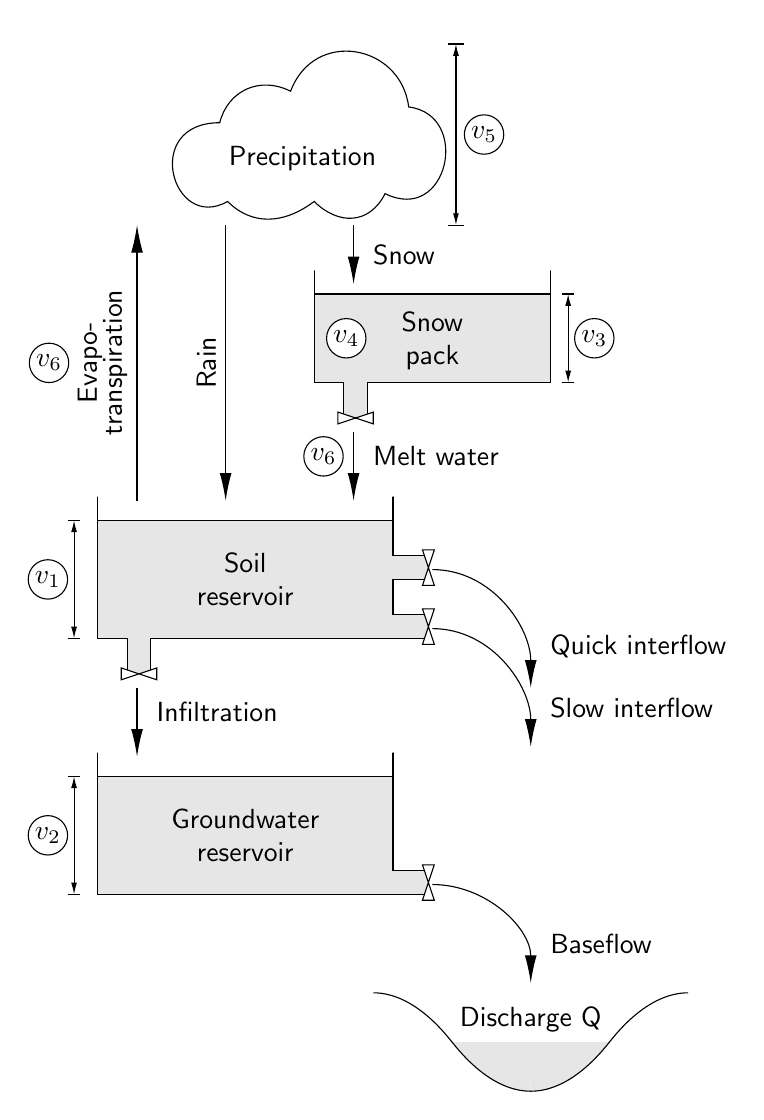
\begin{tikzpicture}[scale=2.5]
		% cloud
		\AsymCloud{(1.0,0.3)}{Precipitation}{0.4}
		
		% arrows rain/snow/snowpack 
		\draw [-{Latex[length=3.5mm, width=1.5mm]}] (0.35,-0.1) -- (0.35,-1.5);
		\node[above,align=center,rotate=90] at (0.35,-0.8) {Rain};
		\draw [-{Latex[length=3.5mm, width=1.5mm]}] (1.0,-0.1) -- (1.0,-0.4);
		\node[right,align=left,rotate=0] at (1.05,-0.25) {Snow};
		%\node[rectangle,draw,align=center,rotate=0,fill=ufzgray4] at (1.0,-0.95) {Snow pack};
		
		% Snow pack
		\BucketWithOneBottomOutlet{(0.8,-0.45)}{Snow\\pack}{0.3}
		
		\draw [-{Latex[length=3.5mm, width=1.5mm]}] (1.0,-1.15) -- (1.0,-1.5);
		\node[right,align=left,rotate=0] at (1.05,-1.275) {Melt water};
		
		\draw [-{Latex[length=3.5mm, width=1.5mm]}] (-0.1,-1.5) -- (-0.1,-0.1);
		\node[above,align=center,rotate=90] at (-0.1,-0.8) {Evapo-\\[-3pt]transpiration};
		
		% variable v_6 = temparture (evapo) 
		\node[draw,right,align=left,circle,minimum size=0.5cm,inner sep=0pt] at (-0.65,-0.8) {\texttt{$v_6$}};
		% variable v_6 = temparture (snow melt) 
		\node[draw,left,align=right,circle,minimum size=0.5cm,inner sep=0pt] at (0.95,-1.275) {\texttt{$v_6$}};
		
		\BucketWithThreeOutlets{(-0.3,-1.6)}{Soil\\reservoir}{0.3}
		
		\draw [-{Latex[length=3.5mm, width=1.5mm]}] (-0.1,-2.45) -- (-0.1,-2.8);
		\node[right,align=left,rotate=0] at (-0.05,-2.575) {Infiltration};
		
		\BucketWithOneSideOutlet{(-0.3,-2.9)}{Groundwater\\reservoir}{0.3}
		
		% long arrow to the right
		%\draw [-{Latex[length=3.5mm, width=1.5mm]}] (1.9,-2.33) -- (1.9,-3.95);
		
		% three outlet arrows
		\draw [-{Latex[length=3.5mm, width=1.5mm]}] (1.4,-1.85) to [out=0,in=90] (1.9,-2.45);
		\node[above right, align=left,rotate=0] at (1.95,-2.35) {Quick interflow};
		\draw [-{Latex[length=3.5mm, width=1.5mm]}] (1.4,-2.15) to [out=0,in=90] (1.9,-2.75);
		\node[above right, align=left,rotate=0] at (1.95,-2.65) {Slow interflow};
		\draw [-{Latex[length=3.5mm, width=1.5mm]}] (1.4,-3.45) to [out=0,in=90] (1.9,-3.95);
		\node[above right, align=left,rotate=0] at (1.95,-3.85) {Baseflow};
		
		% River Discharge
		\RiverDischarge{(1.7,-4.25)}{Discharge Q}{0.2}
		
		%\node[draw, below, align=center,rotate=0,rectangle,fill=white] at (1.9,-4.0) {Discharge Q};
		
	
%		\tikzstyle{block} = [rectangle, draw, fill=white!20, 
%		text width=13em, text centered, rounded corners, minimum height=1em]
%		\tikzstyle{noblock} = [rectangle, fill=white!20, 
%		text width=14em, rounded corners, minimum height=1em]
%		\tikzstyle{abcblock} = [rectangle, fill=white!20, 
%		text width=1em, rounded corners, minimum height=1em]
%		\tikzstyle{line} = [draw, -latex']
%		\tikzstyle{line} = [draw,latex'-latex'new]
%		
%		% caption
%		\node [noblock,align=center] (A) {\textbf{Identification of Recipes}};
%		\node [noblock,align=center,right of=A,xshift=6cm] (B) {\textbf{Application of Recipes}};
%		
%		% ABC
%		\node [abcblock,align=center,left of=A,xshift=-1.55cm] {{\LARGE \textbf{A}}};
%		\node [abcblock,align=center,left of=B,xshift=-1.55cm] {{\LARGE \textbf{B}}};
%		
%		% Identification of Recipes
%		\node [block, below of=A, node distance=1.5cm] (a1) {\textbf{Setup} of CEQUEAU of four basins for years 2011 to 2015 (1826 days)};
%		\node [noblock,rotate=90,align=center,left=0.25cm of a1.west,text width=0.4em,xshift=-0.25cm] (a1sec) {\small Sec.~3.1};
%		
%		\node [block, below=0.64cm of a1.south, node distance=2.5cm] (a2) {\textbf{Analyse} model setups using Efficient Elementary Effects (EEE) to identify informative parameters};
%		\node [noblock,rotate=90,align=center,left=0.46cm of a2.west,text width=0.4em,xshift=-0.25cm] (a2sec) {\small Sec.~3.2\\Sec.~4.1};
%		
%		\node [block, below=0.64cm of a2.south, node distance=2.5cm] (a3) {\textbf{Identify} under which (meteorologic) conditions parameter is informative};
%		\node [noblock,rotate=90,align=center,left=0.46cm of a3.west,text width=0.4em,xshift=-0.25cm] (a2sec) {\small Sec.~3.3\\Sec.~4.1};
%		
%		\node [block, below=0.64cm of a3.south, node distance=2.5cm, fill=ufzgray3] (a4) {\textbf{Proposed Recipe:}\\ Summary of which parameters are informative given a (meteorologic) condition};
%		\node [noblock,rotate=90,align=center,left=0.25cm of a4.west,text width=0.4em,xshift=-0.25cm] (a2sec) {\small Sec.~4.1};
%		
%		\node [block, below=0.84cm of a4.south, node distance=2.5cm, fill=ufzgray4] (a5) {\textbf{Expert Recipe:}\\ Summary of informative parameters given (meteorologic) conditions defined by expert forecasting analyst};
%		\node [noblock,rotate=90,align=center,left=0.25cm of a5.west,text width=0.4em,xshift=-0.25cm] (a2sec) {\small Sec.~4.1};
%		
%		\node [block, below of=B, node distance=1.5cm] (b1) {\textbf{Setup} of CEQUEAU for\\ random day in\\ random basin$^{*}$};
%		\node [noblock,rotate=90,align=center,left=0.25cm of b1.west,text width=0.4em,xshift=-0.25cm] (b2sec) {\small Sec.~3.1};
%				
%		\node [block, below=0.53cm of b1.south, node distance=2.5cm] (b2) {\textbf{Look-up} meteorologic conditions of simulation start day and/or previous days};
%		\node [noblock,rotate=90,align=center,left=0.25cm of b2.west,text width=0.4em,xshift=-0.25cm] (b2sec) {\small Sec.~3.4};
%		
%		\node [block, below=0.53cm of b2.south, node distance=2.5cm, text width=6.em, xshift=-3.5em, fill=ufzgray3] (b3a) {\textbf{Select} informative parameters based on \textbf{Proposed Recipe}};
%		\node [block, below=0.53cm of b2.south, node distance=2.5cm, text width=5.6em, xshift=3.7em, fill=ufzgray4] (b3b) {\textbf{Select} informative parameters based on \textbf{Expert Recipe}};
%		\node [noblock,rotate=90,align=center,left=0.25cm of b3a.west,text width=0.4em,xshift=-0.25cm] (b3sec) {\small Sec.~3.4};
%		
%		\node [block, below=0.53cm of b3a.south, node distance=2.5cm, xshift=3.5em] (b4) {\textbf{Calibrate} CEQUEAU using informative parameters only};
%		\node [noblock,rotate=90,align=center,left=0.25cm of b4.west,text width=0.4em,xshift=-0.25cm] (b4sec) {\small Sec.~3.4};
%		
%		\node [block, below=0.53cm of b4.south, node distance=2.5cm] (b5) {\textbf{Analyze} calibration results to determine performance of recipe};
%		\node [noblock,rotate=90,align=center,left=0.46cm of b5.west,text width=0.4em,xshift=-0.25cm] (b5sec) {\small Sec.~3.5\\Sec.~4.2};
%		
%		\node [block, below=0.53cm of b5.south, node distance=2.5cm] (b6) {\textbf{Forecast} simulations to determine performance of recipe};
%		\node [noblock,rotate=90,align=center,left=0.46cm of b6.west,text width=0.4em,xshift=-0.25cm] (b5sec) {\small Sec.~3.6\\Sec.~4.3};
%		
%		% lines A-B (realistic setup)
%		\draw [-{Latex[length=3.5mm, width=1.5mm]}] (a1.south) -- (a2.north);
%		\draw [-{Latex[length=3.5mm, width=1.5mm]}] (a2.south) -- (a3.north);
%		\draw [-{Latex[length=3.5mm, width=1.5mm]}] (a3.south) -- (a4.north);
%		
%		\draw [-{Latex[length=3.5mm, width=1.5mm]}] (b1.south) -- (b2.north);
%		\draw [-{Latex[length=3.5mm, width=1.5mm]}] (b2.south) -- (b3a.north);
%		\draw [-{Latex[length=3.5mm, width=1.5mm]}] (b2.south) -- (b3b.north);
%		\draw [-{Latex[length=3.5mm, width=1.5mm]}] (b3a.south) -- (b4.north);
%		\draw [-{Latex[length=3.5mm, width=1.5mm]}] (b3b.south) -- (b4.north);
%		\draw [-{Latex[length=3.5mm, width=1.5mm]}] (b4.south) -- (b5.north);
%		\draw [-{Latex[length=3.5mm, width=1.5mm]}] (b5.south) -- (b6.north);
		
	\end{tikzpicture}

\end{document}



